\documentclass{beamer}
\mode<presentation> {
	\usetheme{Boadilla}
	% \usecolortheme{crane}
	% \setbeamercovered{transparent}
	% or whatever (possibly just delete it)
}

\usepackage[T2A]{fontenc}
\usepackage[utf8]{inputenc}
\usepackage[bulgarian]{babel}
\usepackage{amsmath}
\usetheme{default}

\newtheorem{thm}{Теорема}
\newtheorem{cor}[thm]{Следствие}
\newtheorem{lem}[thm]{Лема}
\newtheorem{prop}[thm]{Твърдение}

\theoremstyle{definition}
\newtheorem{defn}[thm]{Дефиниция}
\newtheorem{nabl}[thm]{Наблюдение}
\newtheorem{krpl}[thm]{Критична плътност}

\newtheorem{defnplt}[thm]{Дефиниция за плътност в конкретната задача}
\newtheorem{gammaform}[thm]{Формула за $\gamma$}
\newtheorem{kgammaform}[thm]{Формула за $k_{\gamma}$}
\newtheorem{ksr}[thm]{Формула за $k_{_{\scriptstyle\text{ср.}}}$ (типичното количество памет)}
\newtheorem{pnk}[thm]{Формула за $p_{n\,;\,k}$}
\newtheorem{pkr}[thm]{Формула за $p_{_{_{\scriptstyle\text{кр.}}}}$}
\newtheorem{ksrkrit}[thm]{Типично количество памет за графи с критична плътност}
\newtheorem{ksrkrit2}[thm]{Типично количество памет за дъски с критична плътност}
\newtheorem{graphalg}[thm]{Резултати от тестването на алгоритъма}
\newtheorem{prblpnp}[thm]{Приблизителна формула за $P_n(p)$ }
\newtheorem{hypqueens}[thm]{Хипотеза на Беноа Кльоатър}
\theoremstyle{remark}
\newtheorem*{rem}{Забележка}

\title[Търсене с връщане]{Стохастичен анализ на количеството памет\\ на алгоритмичната схема търсене с връщане}
\author{Ангел Димитриев}
\date{СУ, ФМИ, 2022 г.}
\begin{document}
\begin{frame}[plain]
	\maketitle
\end{frame}
\begin{frame}{Увод --- типично количество памет}
	От практическа гледна точка не е проблем, ако една програма\\
	се нуждае от много памет временно, стига да използва малко памет\\
   	през повечето време от своята работа. Ето защо е съществено\\
	не толкова максималното, колкото типичното количество памет,\\
	използвано от програмата по време на изпълнение.
	\begin{defn} 
		Под типично количество памет разбираме онази стойност,\\
		около която се колебае използваното количество памет\\
		през по-голямата част от времето за изпълнение на програмата.
	\end{defn}
	Типичното количество памет зависи от:\\
	$\bullet$ обема на входните данни;\\
	$\bullet$ плътността на входните данни\\ (различна дефиниция за всяка задача).
\end{frame}
\begin{frame}{Увод --- избор на мярка}
	За мярка на паметта избираме \textbf{текущия брой елементи}\\
	\textbf{на построявания комбинаторен обект}. Бележим с $\xi$.\\
	Тъй като величината  $\xi$ се мени с изпълнението на алгоритъма,\\
	ще я бележим с $\xi_{\,t}$ , където индексът $t$ означава \textbf{текущия момент}.\\
	Използваме модел с дискретно време: $t\in\{\,0\,;\,1\,;\,2\,;\,\ldots\,;\,T\,\}$,\\
	където $T$ е броят на всички стъпки на алгоритъма.
	\begin{nabl} 
		\mbox{$\xi_{\,0} = 0$}\, за всякакви входни данни, а
		\mbox{$\xi_{\,T} = n$}\, за входни данни,\\
		при които търсеният обект съществува.
	\end{nabl}			
	Входните данни $\omega$ се избират случайно. 
	При това тълкуване \mbox{$\xi_{\,t}=\xi_{\,t}(\omega)$}\\
	се превръща в \textbf{случайна величина} за произволно, но фиксирано $t$;\\
	а когато $t$ пробягва целите числа от $0$ до $T$,
	се получава редицата\\ \mbox{$\left(\xi_{\,t}\right)_{t\geq 0}$,}
	която представлява \textbf{случаен процес}.
	Неговите числови\\ характеристики
	са основен интерес на настоящото изследване.
\end{frame}
\begin{frame}{Модел за пресмятане на типично количество памет}
	При търсене с връщане важи формулата\,
    \mbox{$\xi_{\,t+1} = \xi_{\,t} \pm 1$.}
	\begin{defn}
		$p_{n\,;\,k} = \mathbf{P}\bigl\{\xi_{\,t+1} = k - 1 \mid \xi_{\,t} = k \bigr\}$
		е вероятността $\xi$ да намалее,\\
		вместо да се увеличи (зависи от $n$, $p$ и от текущата стойност $k$ на $\xi$).
	\end{defn}
	Обикновено $p_{n\,;\,k}$ е растяща функция на $k$.\\
	Конкретната функция се различава от задача към задача.
	\begin{defn} 
		Обратната функция на $p_{n\,;\,k}$ бележим с  $k_{\gamma}$, тоест\\
		$p_{n\,;\,k} = \gamma   \iff   k = k_{\gamma}$ (като функция на $\gamma$, $n$ и $p$).
	\end{defn}	
\end{frame}
\begin{frame}{Модел за пресмятане на типично количество памет}
	\begin{defn}
		Равновесна точка --- \mbox{$k_{_{\scriptstyle 0,5}}$.}
	\end{defn}
	В околност на равновесната точка\\
	процесът $\xi_{\,t}$ има характер на симетрично случайно лутане.\\
	\mbox{}\,\\
	Нужен ни е критерий, по който да изберем
	околността на равновесната\\ точка, в която околност да ограничим
	симетричното случайно лутане,\\ но така, че да наподобява процеса $\xi$
	(в смисъл на равенство\\ на математическите очаквания).
\end{frame}
\begin{frame}{Избор на околност на равновесната точка}
	$\bullet$ Връщащата сила трябва да е еднаква в двата края, затова търсим\\
	интервал от вида
    \mbox{$[k_{_{\scriptstyle 1-\gamma}}\,;\,k_{_{\scriptstyle\gamma}}],\;\;\gamma\in(0,5\,;\,1)$.}\\
	$\bullet$ Дължината на този интервал (в който се извършва лутането)\\
	след подходящо мащабиране трябва да съвпадне с дължината $n$\\
	на интервала от $0$ до $n$, в който се изменя процесът $\xi_{\,t}$.	
	\begin{defn} 
		Мащабен множител $\mu = \mu(k)$:\;\; $p_{n, k} = \left(\dfrac{1}{2}\right)^{\mu}\!.$
	\end{defn}
	Ако процесът \mbox{$\left(\xi_{\,t}\right)_{t\geq 0}$}
	извърши стъпка наляво от точката \mbox{$k$,}\\
	това съответства по вероятност на $\mu(k)$ стъпки наляво\\
	на симетричното случайно лутане.\vspace{-0.8\baselineskip}
	\[
		\sum_{k\,=\,k_{_{\scriptstyle 1-\gamma}}+1}^{k_{_{\scriptstyle\gamma}}}\mu(k)=n,
		\,\text{ тоест }\,
		\sum_{k\,=\,k_{_{\scriptstyle 1-\gamma}}+1}^{k_{_{\scriptstyle\gamma}}}\log_{_{\scriptstyle\,2}}p_{n\,;\,k}=-n.
		\vspace{-0.5\baselineskip}
	\]
	Решението на това уравнение ни дава $\gamma$ като функция на $n$ и $p$.
\end{frame}
\begin{frame}
	В околност на точката \mbox{$k_{_{\scriptstyle 0,5}}$}
	случайният процес има характер\\
	на симетрично случайно лутане, ограничено в интервала
    \mbox{$[k_{_{\scriptstyle 1-\gamma}}\,;\,k_{_{\scriptstyle\gamma}}]$.}\\
	Това лутане може да се представи чрез верига на Марков:\vspace{\baselineskip}\\
	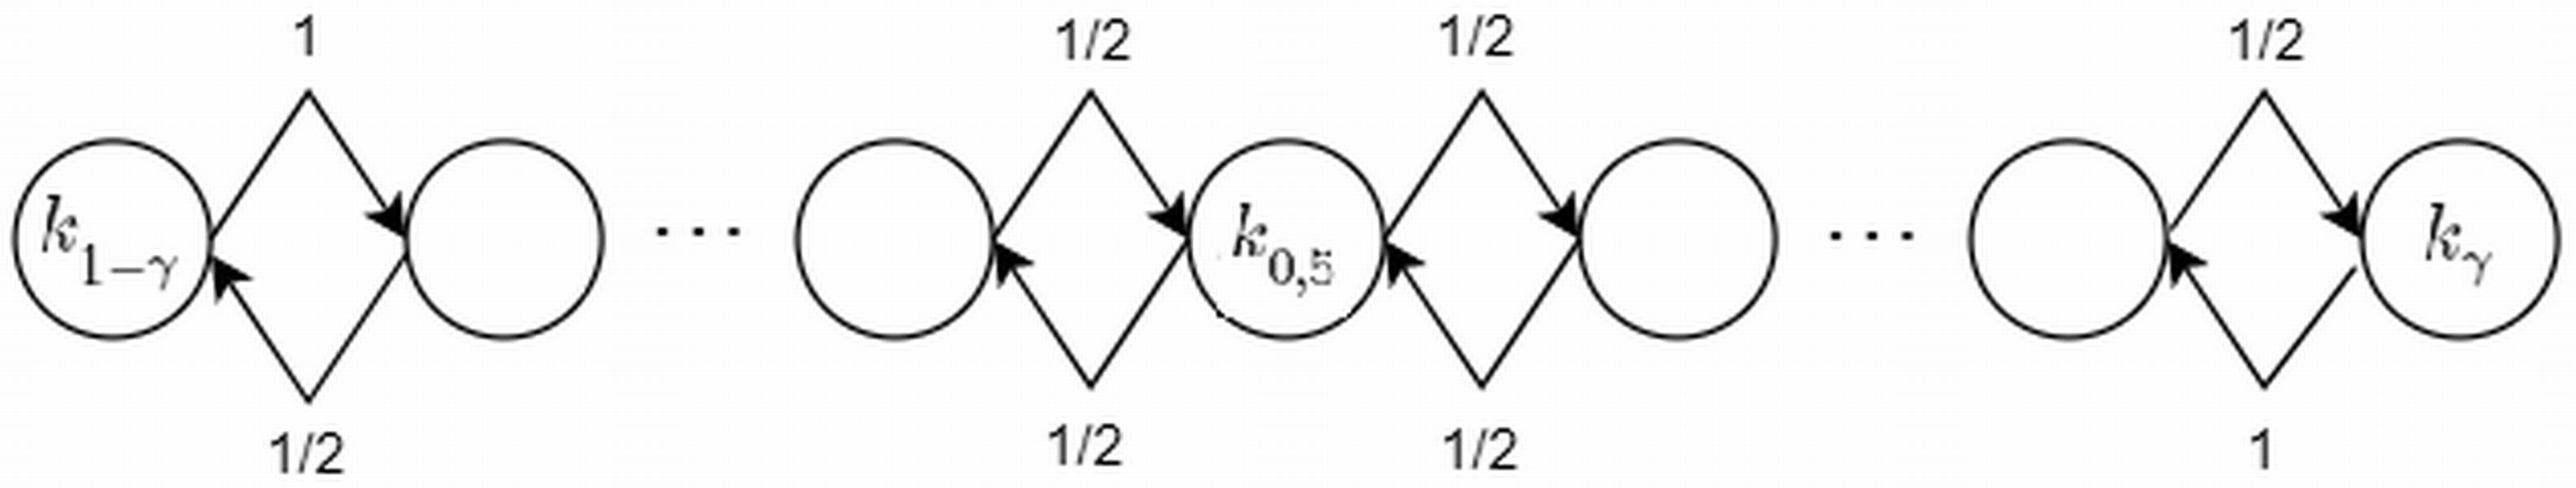
\includegraphics[scale=0.11]{MarkovChain.png}\vspace{\baselineskip}\\
	Тази верига е:\\
	$\bullet$ крайна (интервалът съдържа краен брой цели числа);\\
	$\bullet$ еднородна (вероятностите за преход не се менят);\\
	$\bullet$ неразложима (всяка стойност е достижима от всяка друга).\\
	Веригата не е апериодична: има два циклични подкласа\\
	(четните и нечетните числа). Веригите, породени от подкласовете,\\
	са \textbf{ергодични}.
\end{frame}
\begin{frame}
	Разглеждаме една от веригите. След като веригата е ергодична,\\
	тя притежава гранично и единствено стационарно разпределение $\pi$\\
	и те съвпадат. Понеже $\pi$ е стационарно разпределение, то

	\[\pi_{k}=\frac{1}{2}\pi_{k}+\frac{1}{4}\pi_{k-2}+\frac{1}{4}\pi_{k+2}\hspace{1pt},\]

	\[\pi_{k}=\frac{1}{2}\pi_{k-2}+\frac{1}{2}\pi_{k+2}\hspace{1pt}.\]

	Тази редица е аритметична прогресия. Лутането е симетрично,\\
	следователно вероятностите в краищата на интервала са равни.\\
	Затова редицата е константна, тоест $\pi$ е равномерно разпределение\\
	и математическото му очакване е средата $k_{_{\scriptstyle\text{ср.}}}$ на интервала:

	\[k_{_{\scriptstyle\text{ср.}}}=\frac{1}{2}\left(k_{_{\scriptstyle 1-\gamma}}+k_{_{\scriptstyle\gamma}}\right)\]

	е \textbf{типичното количество използвана памет}. 
\end{frame}
\begin{frame}{Търсене на хамилтонов цикъл}
	Разглеждаме известната задача за търсене на хамилтонов цикъл\\
	в даден неориентиран граф с $n$ върха.
	Тълкуваме входните данни\\ като случаен граф:
	за всеки два различни върха вероятността да има\\ ребро между тях
	е някакво реално число \mbox{$p\in[0\,;\,1]$} --- 
	едно и също\\ за всеки два върха.\\
	\begin{defnplt} 
		Вероятността $p$ за съществуване на ребро между два произволни\\
		върха в графа наричаме \textbf{плътност} на графа.
	\end{defnplt}
	\begin{defn} 
		$P_n(p)$ е вероятността за съществуване на хамилтонов цикъл.
	\end{defn}
	\begin{nabl} 
		\mbox{$P_n(0) = 0$,} \;\mbox{$P_n(1) = 1$}\; и\;
		$P_n(p)$ е растяща функция на $p$.
	\end{nabl}
\end{frame}
\begin{frame}{Търсене на хамилтонов цикъл (експерименти)}
	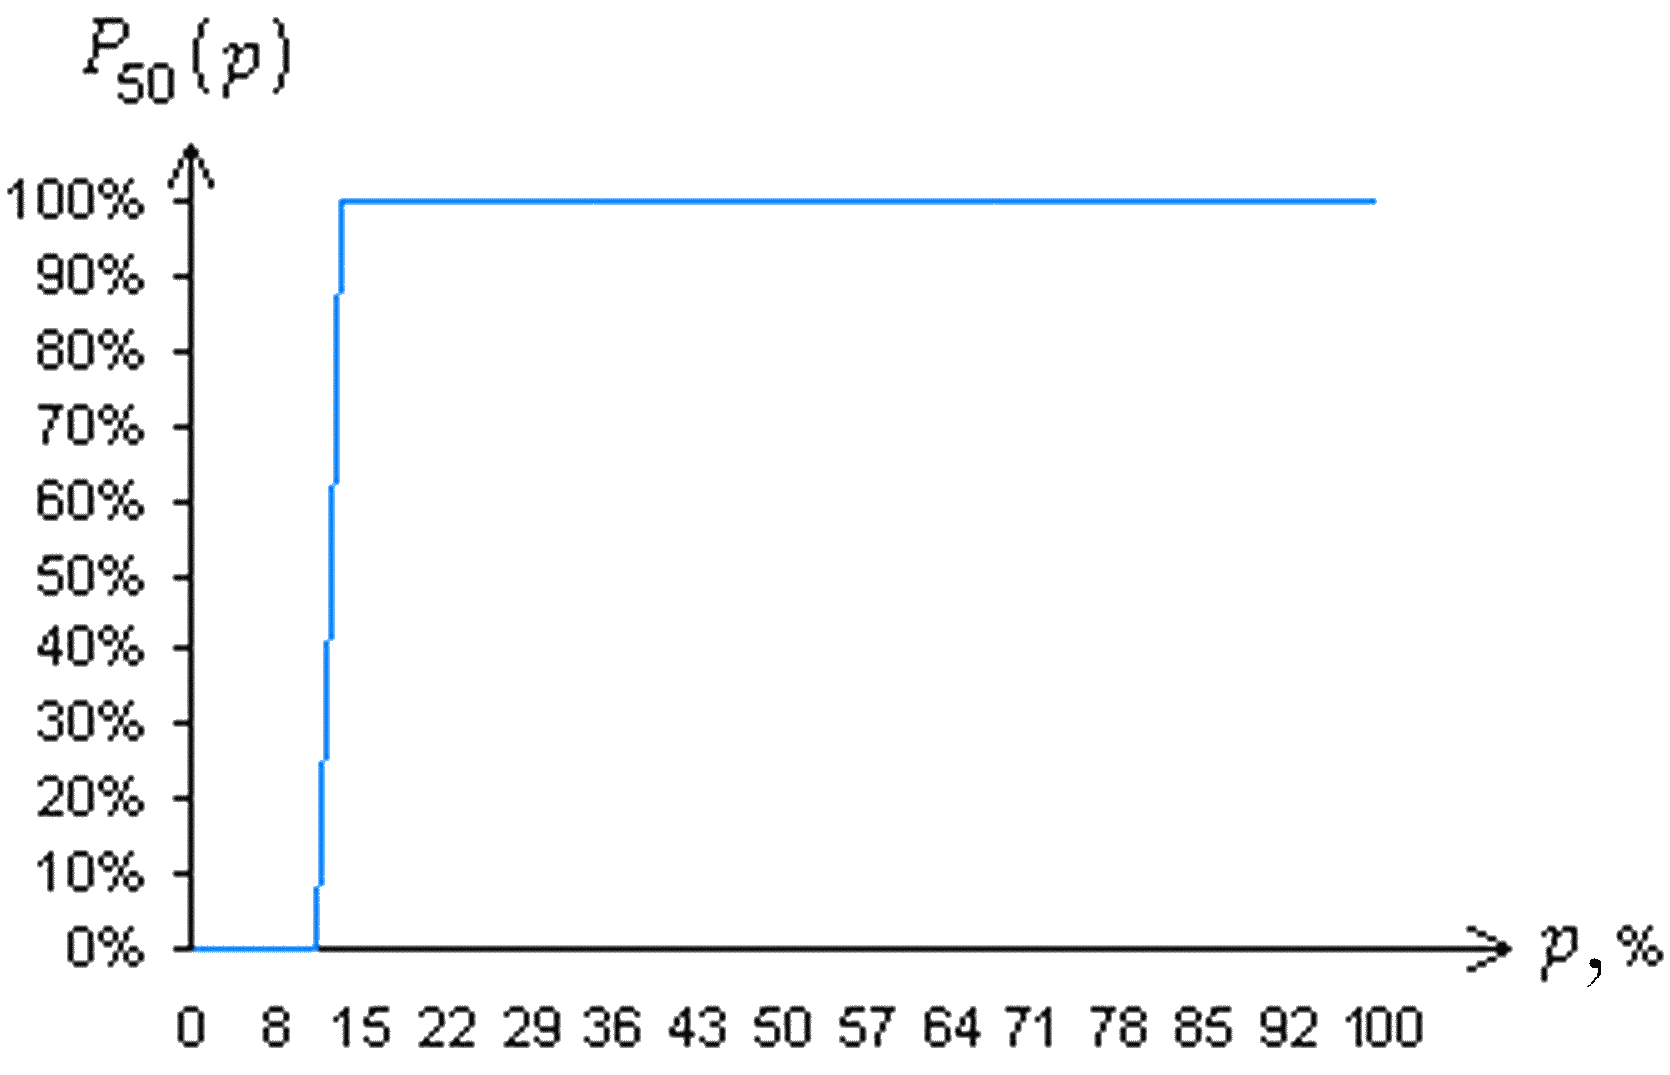
\includegraphics[scale=0.10]{ham50.png}\\
	Експериментите показват, че $P_n(p)$ расте стръмно от 0 до 1.\\
	Например \mbox{$P_{50}(0,11) < 0,01$} и \mbox{$P_{50}(0,14) > 0,99$,}
	тоест почти цялото\\ нарастване на $P_n(p)$ от 0 до 1
	се извършва, когато плътността $p$\\
    се мени от 0,11 до 0,14 --- участък с ширина едва 0,03.\\
	Извън критичния участък можем да си спестим търсенето, приемайки,\\
	че има хамилтонов цикъл за $p$ надясно от критичния участък,\\
	няма хамилтонов цикъл за $p$ наляво от този участък.
\end{frame}
\begin{frame}{Търсене на хамилтонов цикъл (експерименти)}
	\begin{defn} 
		Критична плътност:\; $P_n\left(p_{_{_{\scriptstyle\text{кр.}}}}\right) = \frac{1}{2}\hspace{1pt}\cdot$
	\end{defn}
	При графи с критична плътност търсенето работи бавно,\\
	ето защо е важно колко памет изразходва.\vspace{0.2\baselineskip}\\
	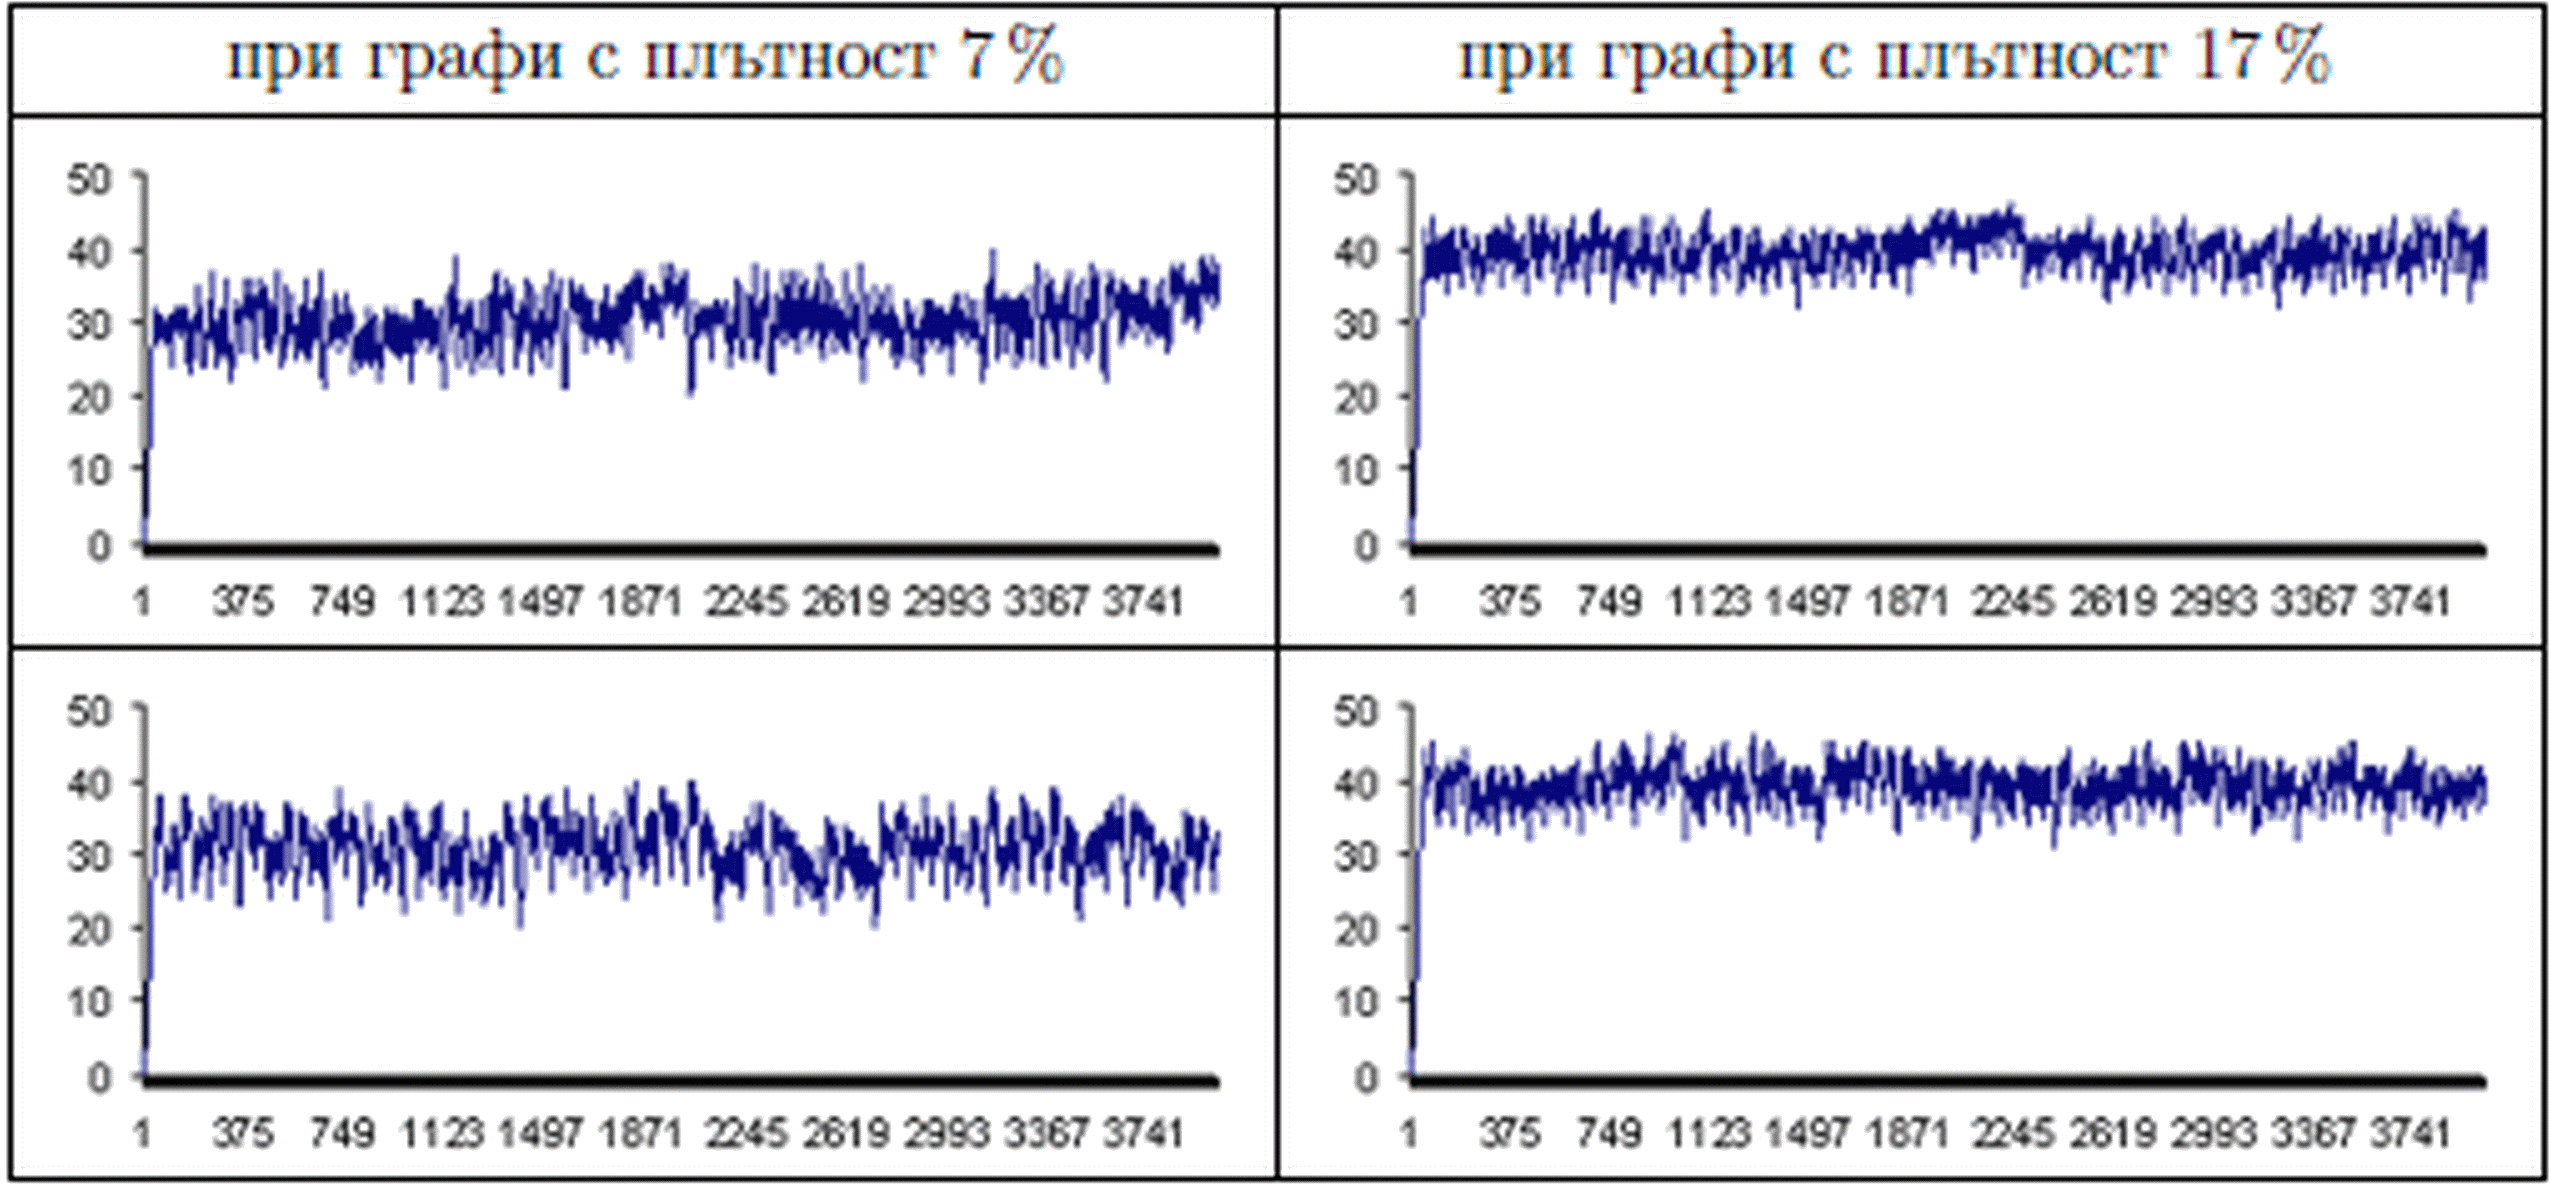
\includegraphics[scale=0.11]{ham717.png}
\end{frame}
\begin{frame}{Търсене на хамилтонов цикъл (експерименти)}
	--- При плътност 7\,\% почти всички графи са нехамилтонови:\\
	\mbox{}\phantom{--- }26,9;\: 25,3;\: 35,4;\: 32,4;\: 31,0;\: 21,8;\: 29,8;\: 31,9;\: 22,2.\\
	\mbox{}\phantom{--- }Числови характеристики:\\
	\mbox{}\phantom{--- }обем: $n_x = 9$;\\
	\mbox{}\phantom{--- }средноаритметично: $\overline{x} = 28,5$;\\
	\mbox{}\phantom{--- }средно отклонение: $s_x = 4,7$.\medskip\\
	--- При плътност 17\,\% почти всички графи са хамилтонови:\\
	\mbox{}\phantom{--- }44,0;\: 42,4;\: 37,8;\: 44,6;\: 41,1;\: 42,8;\: 40,8;\: 39,2;\: 39,2.\\
	\mbox{}\phantom{--- }Числови характеристики:\\
	\mbox{}\phantom{--- }обем: $n_y = 9$;\\
	\mbox{}\phantom{--- }средноаритметично: $\overline{y} = 41,3$;\\
	\mbox{}\phantom{--- }средно отклонение: $s_y = 2,3$.\medskip\\
	Статистиката $T'$ показва, че има статистически значима разлика\\
	между средните стойности:\, типичното количество памет расте\\
	с увеличаване на плътността на графа.
\end{frame}
\begin{frame}{Търсене на хамилтонов цикъл}
	\begin{krpl} 
		\mbox{$p_{_{_{\scriptstyle\text{кр.}}}}\sim\,\dfrac{\ln n}{n}$}\; (теорема на Поза, уточнена от Коршунов).\medskip
	\end{krpl}
	По правилото за умножение намираме
	\[\mathbf{P}\bigl\{\xi_{\,t+1} = \xi_{\,t} - 1 \;\bigr|\bigl.\;\xi_{\,t} = k\bigr\} = p_{n\,;\,k}=(1-p)^{n-k},\;\;1 \leq k \leq n.\]
    Тъй като случайният процес е ограничен между $0$ и $n$ вкл.:
    
	$\bullet$ \mbox{$p_{n\,;\,0}=0$;}\\
	
	$\bullet$ \mbox{$p_{n\,;\,n}=1$.}\\
	\begin{pnk} 
		\mbox{$p_{n\,;\,k} =
		\left\{\begin{tabular}{ll}$0$, & $k = 0$;\\$(1-p)^{n-k}$, & $1 \leq k \leq n$.\end{tabular}\right.$}
	\end{pnk}
\end{frame}
\begin{frame}{Търсене на хамилтонов цикъл}
	Решаваме относно $k$ уравнението
	\mbox{$p_{n\,;\,k}=\gamma$,}
	тоест \mbox{$(1-p)^{n-k}=\gamma$,}\\
	и намираме \mbox{$k = n - \log_{1-p}\gamma$.}
	\begin{kgammaform} 
		\[k_{_{\scriptstyle\gamma}} = n - \frac{\ln\gamma}{\ln(1-p)}\hspace{1pt}\cdot\]
	\end{kgammaform}
	Търсим подходящ интервал 
    \mbox{$[k_{_{\scriptstyle 1-\gamma}}\,;\,k_{_{\scriptstyle\gamma}}],\;\;\gamma\in(0,5\,;\,1)$:}\\
	\[\sum_{k\,=\,k_{_{\scriptstyle 1-\gamma}}+1}^{k_{_{\scriptstyle\gamma}}}\log_{_{\scriptstyle\,2}}(1-p)^{n-k}=-n.\]
	\begin{gammaform} 
		\[\gamma\approx 1-\exp\left(-\,\sqrt{-2n\,.\,\ln 2\,.\,\ln(1-p)}\,\right)\!.\]
	\end{gammaform}
\end{frame}
\begin{frame}{Търсене на хамилтонов цикъл}
	\begin{ksr}
		\[k_{_{\scriptstyle\text{ср.}}}=\frac{1}{2}\left(k_{_{\scriptstyle 1-\gamma}}+k_{_{\scriptstyle\gamma}}\right) = n-\frac{\ln\Bigl(\gamma(1-\gamma)\Bigr)}{2\,\ln(1-p)}\]
	\end{ksr}	
	е \textbf{типичното количество използвана памет} --- равнището,\\
	около което се колебаят стойностите на случайния процес\\
	във водоравния участък на траекторията.\\
	При \mbox{$p_{_{_{\scriptstyle\text{кр.}}}}\sim\,\dfrac{\ln n}{n}$} получаваме:
	\begin{ksrkrit} 
		\[k_{_{\scriptstyle\text{ср.}}}\approx n\left(1-\sqrt{\frac{0,5\,.\,\ln 2}{\ln n}}\right)\!\cdot\]
	\end{ksrkrit}	
\end{frame}
\begin{frame}{Алгоритъм за разпознаване на хамилтонови графи }
	Оттук произтича следният алгоритъм за разпознаване:\\
	1) Пускаме стандартния алгоритъм за търсене с връщане,\\
	\hspace*{\parindent}\phantom{1)} като следим стойностите
	на случайния процес \mbox{$\xi_{\,t}$.}\\
	2) Щом започне водоравният участък на траекторията,\\
	\hspace*{\parindent}\phantom{2)} образуваме извадка
	от достатъчно стойности на процеса.\\
	3) Пресмятаме средното аритметично $\overline{\xi}$ на извадката.\\
	4) Ако \mbox{$\overline{\xi}>k_{_{\scriptstyle\text{ср.}}}$,}
	приемаме, че графът е хамилтонов;\\
	\hspace*{\parindent}\phantom{4)} в противен случай
	приемаме, че графът не е хамилтонов.\\
	
	Разпознаването на началото на водоравния участък може да стане\\
	с проверка на хипотези за знаците на нарастванията.\\
	Обемът на извадката от водоравния участък може да се намери\\
	по формулата за планиране на обема: \mbox{$\Theta(n)$.}
	\begin{graphalg} 
		Алгоритъмът разпознава правилно $99,9937\,\%$ от графите,
		а останалите\\ $0,0063\,\%$ са разпределени поравно
		между двата типа грешки.
	\end{graphalg}	
\end{frame}
\begin{frame}{Задача за цариците}
	Броя на решенията върху шахматна дъска \mbox{$n \times n$}
	означаваме с \mbox{$\text{Q}(n)$.}
	\begin{hypqueens}
		\[\text{Q}(n)\sim\frac{n!}{c^{\,n}}\,,\quad c \approx 2,54.\]
	\end{hypqueens}
	Ще генерираме входните данни по случаен начин, като всяко поле\\
	ще бъде разрешено с вероятност $p$ независимо от другите полета.\\
	Допустими стойности: \,\mbox{$p\in[0\,;\,1]$.}	
	\begin{defnplt} 	
		Вероятността $p$ случайно избрано поле да бъде разрешено\\
		ще наричаме \textbf{плътност на дъската}.
	\end{defnplt}	
\end{frame}
\begin{frame}{Задача за цариците (експерименти)}
	$P_n(p)=$ вероятността за съществуване на разположение на $n$ царици,\\
	без да се бият, върху шахматна дъска \mbox{$n \times n$} с плътност $p$.\\
	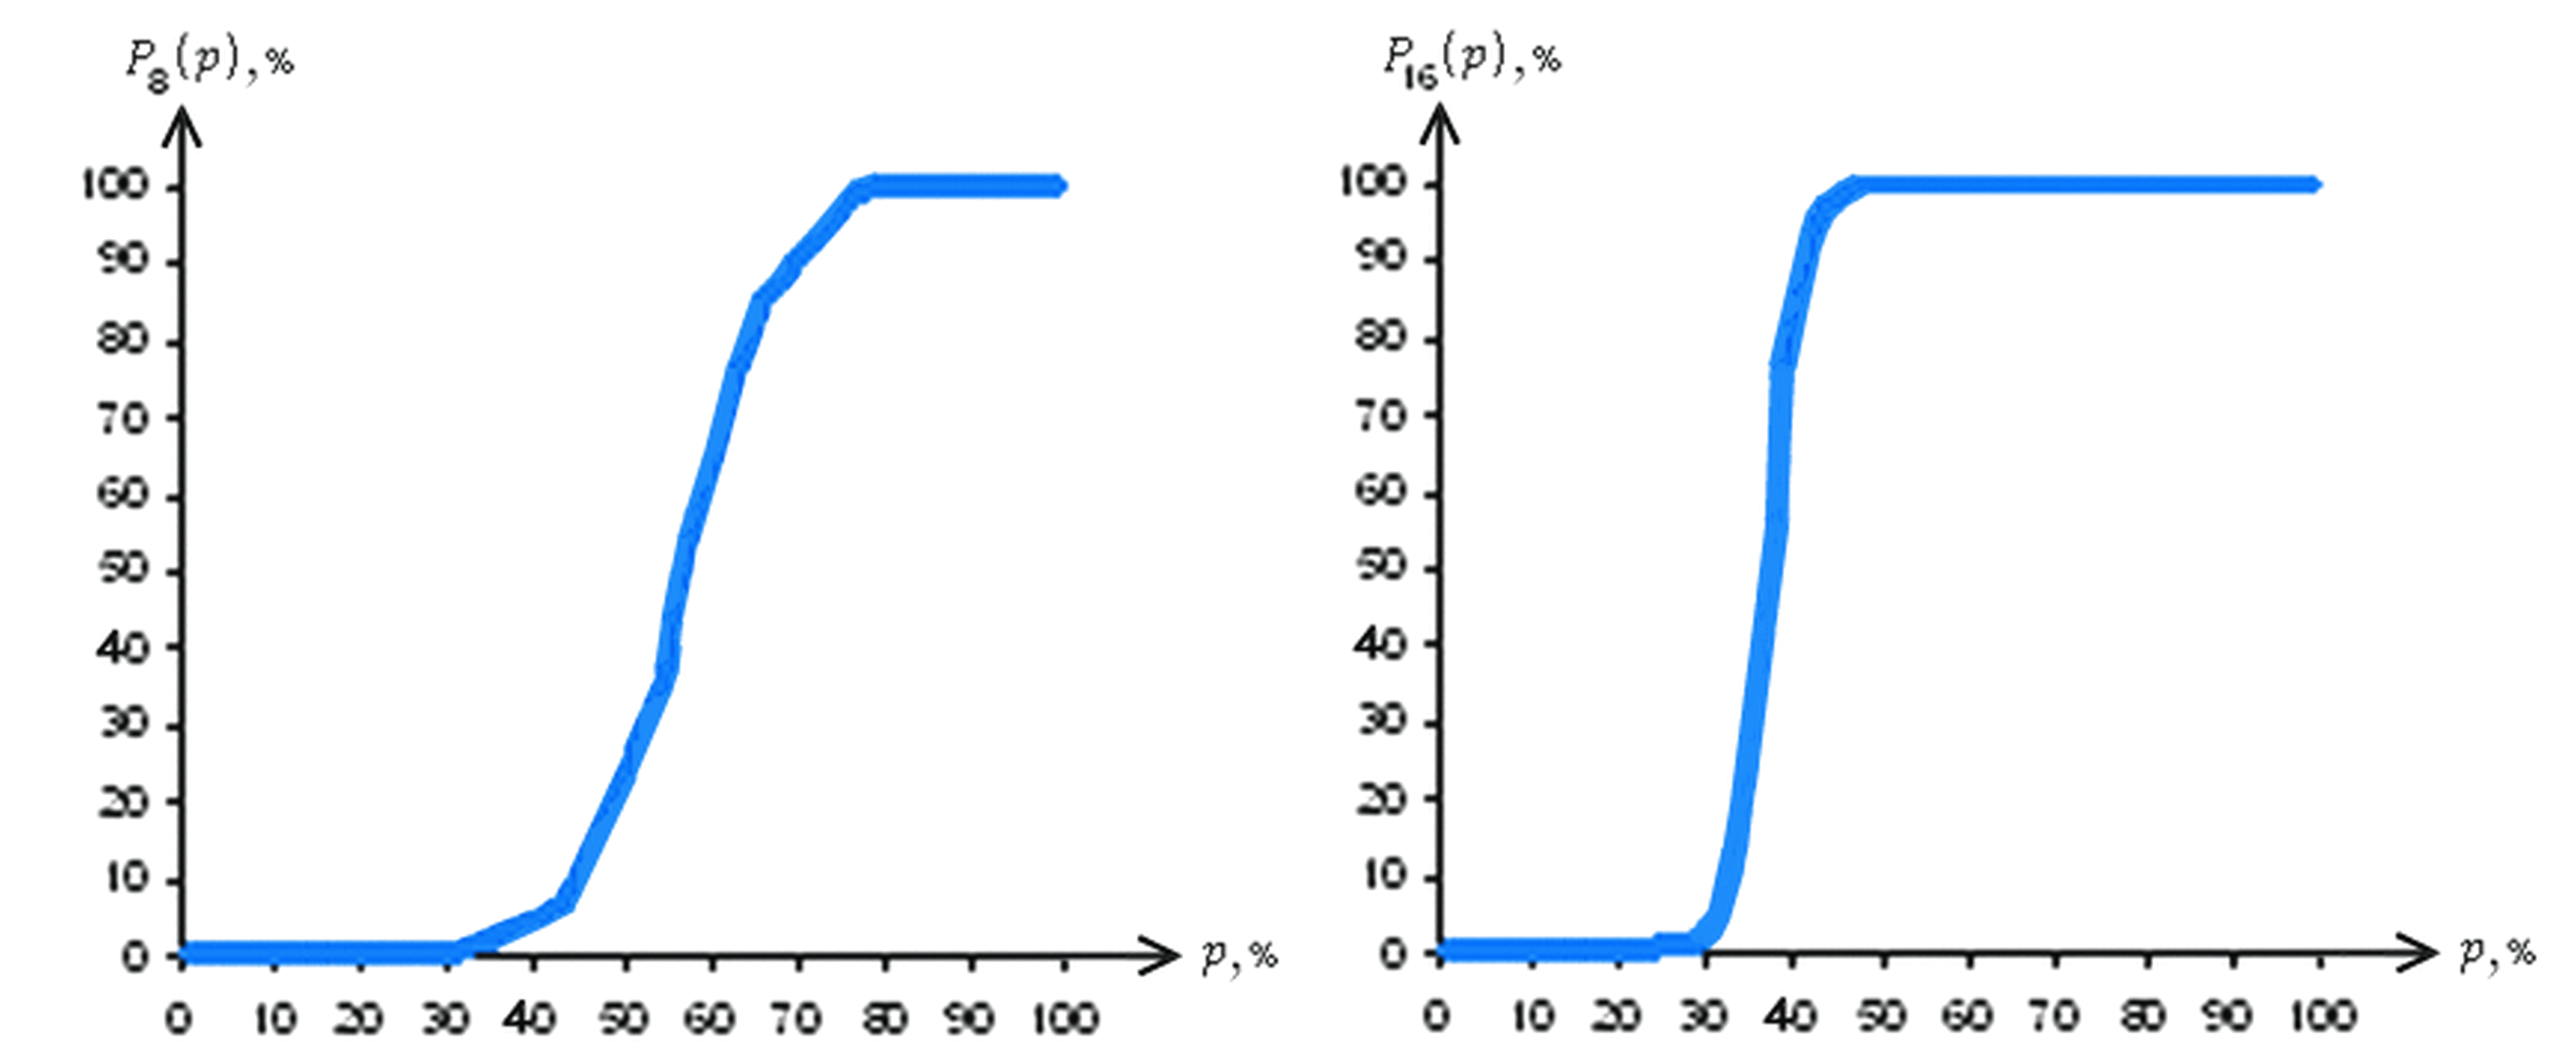
\includegraphics[scale=0.08]{queen_experiments.png}\\
	Задачата е интересна само за
	\mbox{$p \approx p_{_{_{\scriptstyle\text{кр.}}}} = P_n^{-1}(0,5).$}\\
	При задачата за цариците липсва аналог на теоремата на Поза\\
	(асимптотична формула за критичната плътност на дъската).
\end{frame}
\begin{frame}{Задача за цариците }
	Всяко поле независимо от другите остава разрешено с вероятност $p$.\\
	Вероятността да отпадне едно конкретно разположение е \,\mbox{$1-p^{\,n}$.}
	Вероятността да отпаднат всички разположения на цариците\vspace{3pt}\linebreak
	е приблизително \,\mbox{$\left(1-p^{\,n}\right)^{\text{Q}(n)}$.}
	\begin{prblpnp} 	
		\[P_n(p) \approx 1-\left(1-p^{\,n}\right)^{\text{Q}(n)}\]
		е вероятността да съществува поне едно разположение на $n$ царици.
	\end{prblpnp}
	От уравнението \mbox{$P_n\left(p_{_{_{\scriptstyle\text{кр.}}}}\right)=0,5$}
	намираме критичната плътност.
	\begin{pkr} 	
		\[p_{_{_{\scriptstyle\text{кр.}}}}\approx\frac{7}{n}\hspace{1pt}\cdot\]
	\end{pkr}
\end{frame}
\begin{frame}{Задача за цариците}
	\[p_{n\,;\,k}\;=\hspace*{-13pt}\raisebox{3pt}{$^\text{def}$}\;\:\mathbf{P}\bigl\{\xi_{\,t+1} = \xi_{\,t} - 1 \;\bigr|\bigl.\;\xi_{\,t} = k\bigr\}=\mathbf{P}\bigl\{\xi_{\,t+1} = k - 1 \;\bigr|\bigl.\;\xi_{\,t} = k\bigr\}.\]
	\begin{pnk} 	
		\[p_{n\,;\,k}\approx\left(1-\hspace{1pt}p\left(1-\dfrac{k}{n}\right)^{\!3\,}\right)^{\!\!n}.\]
	\end{pnk}
    От уравнението \mbox{$p_{n\,;\,k}=\gamma$} намираме \mbox{$k=k_{_{\scriptstyle\gamma}}$.}
	\begin{kgammaform} 	
		\[k_{_{\scriptstyle\gamma}} \approx n\left(1-\sqrt[3]{\frac{1-\gamma\raisebox{3pt}{$^{1/n}$}}{p}}\;\right)\!\cdot\]
	\end{kgammaform}
\end{frame}
\begin{frame}{Задача за цариците }
	Разглеждаме плътности около критичната.
	\begin{kgammaform} 	
		\[k_{_{\scriptstyle\gamma}} \approx n\left(1+\sqrt[3]{\frac{\ln\gamma}{7}}\;\right)\!.\]
	\end{kgammaform}
	Параметърът $\gamma$
	може да се намери от уравнението\vspace{-0.5\baselineskip}
	\[
		\sum_{k\,=\,k_{_{\scriptstyle 1-\gamma}}+1}^{k_{_{\scriptstyle\gamma}}}\log_{_{\scriptstyle\,2}}p_{n\,;\,k}=-n.\quad
		\text{Получаваме }\,\gamma \approx 0,96979.\vspace{-0.8\baselineskip}
	\] 
	\begin{ksrkrit2} 	
		\[k_{_{\scriptstyle\text{ср.}}}=\frac{1}{2}k_{_{\scriptstyle\gamma}}+\frac{1}{2}k_{_{\scriptstyle 1-\gamma}}\hspace{1pt} \approx \frac{n}{2}\hspace{1pt}\cdot\]
	\end{ksrkrit2}
\end{frame}
\begin{frame}{Задача за цариците (експерименти)}
	Траектории на \mbox{$\left(\xi_{\,t}\right)_{t\geq 0}$}
	при дъска \mbox{$8 \times 8$} с критична плътност.\vspace{3pt}\\
	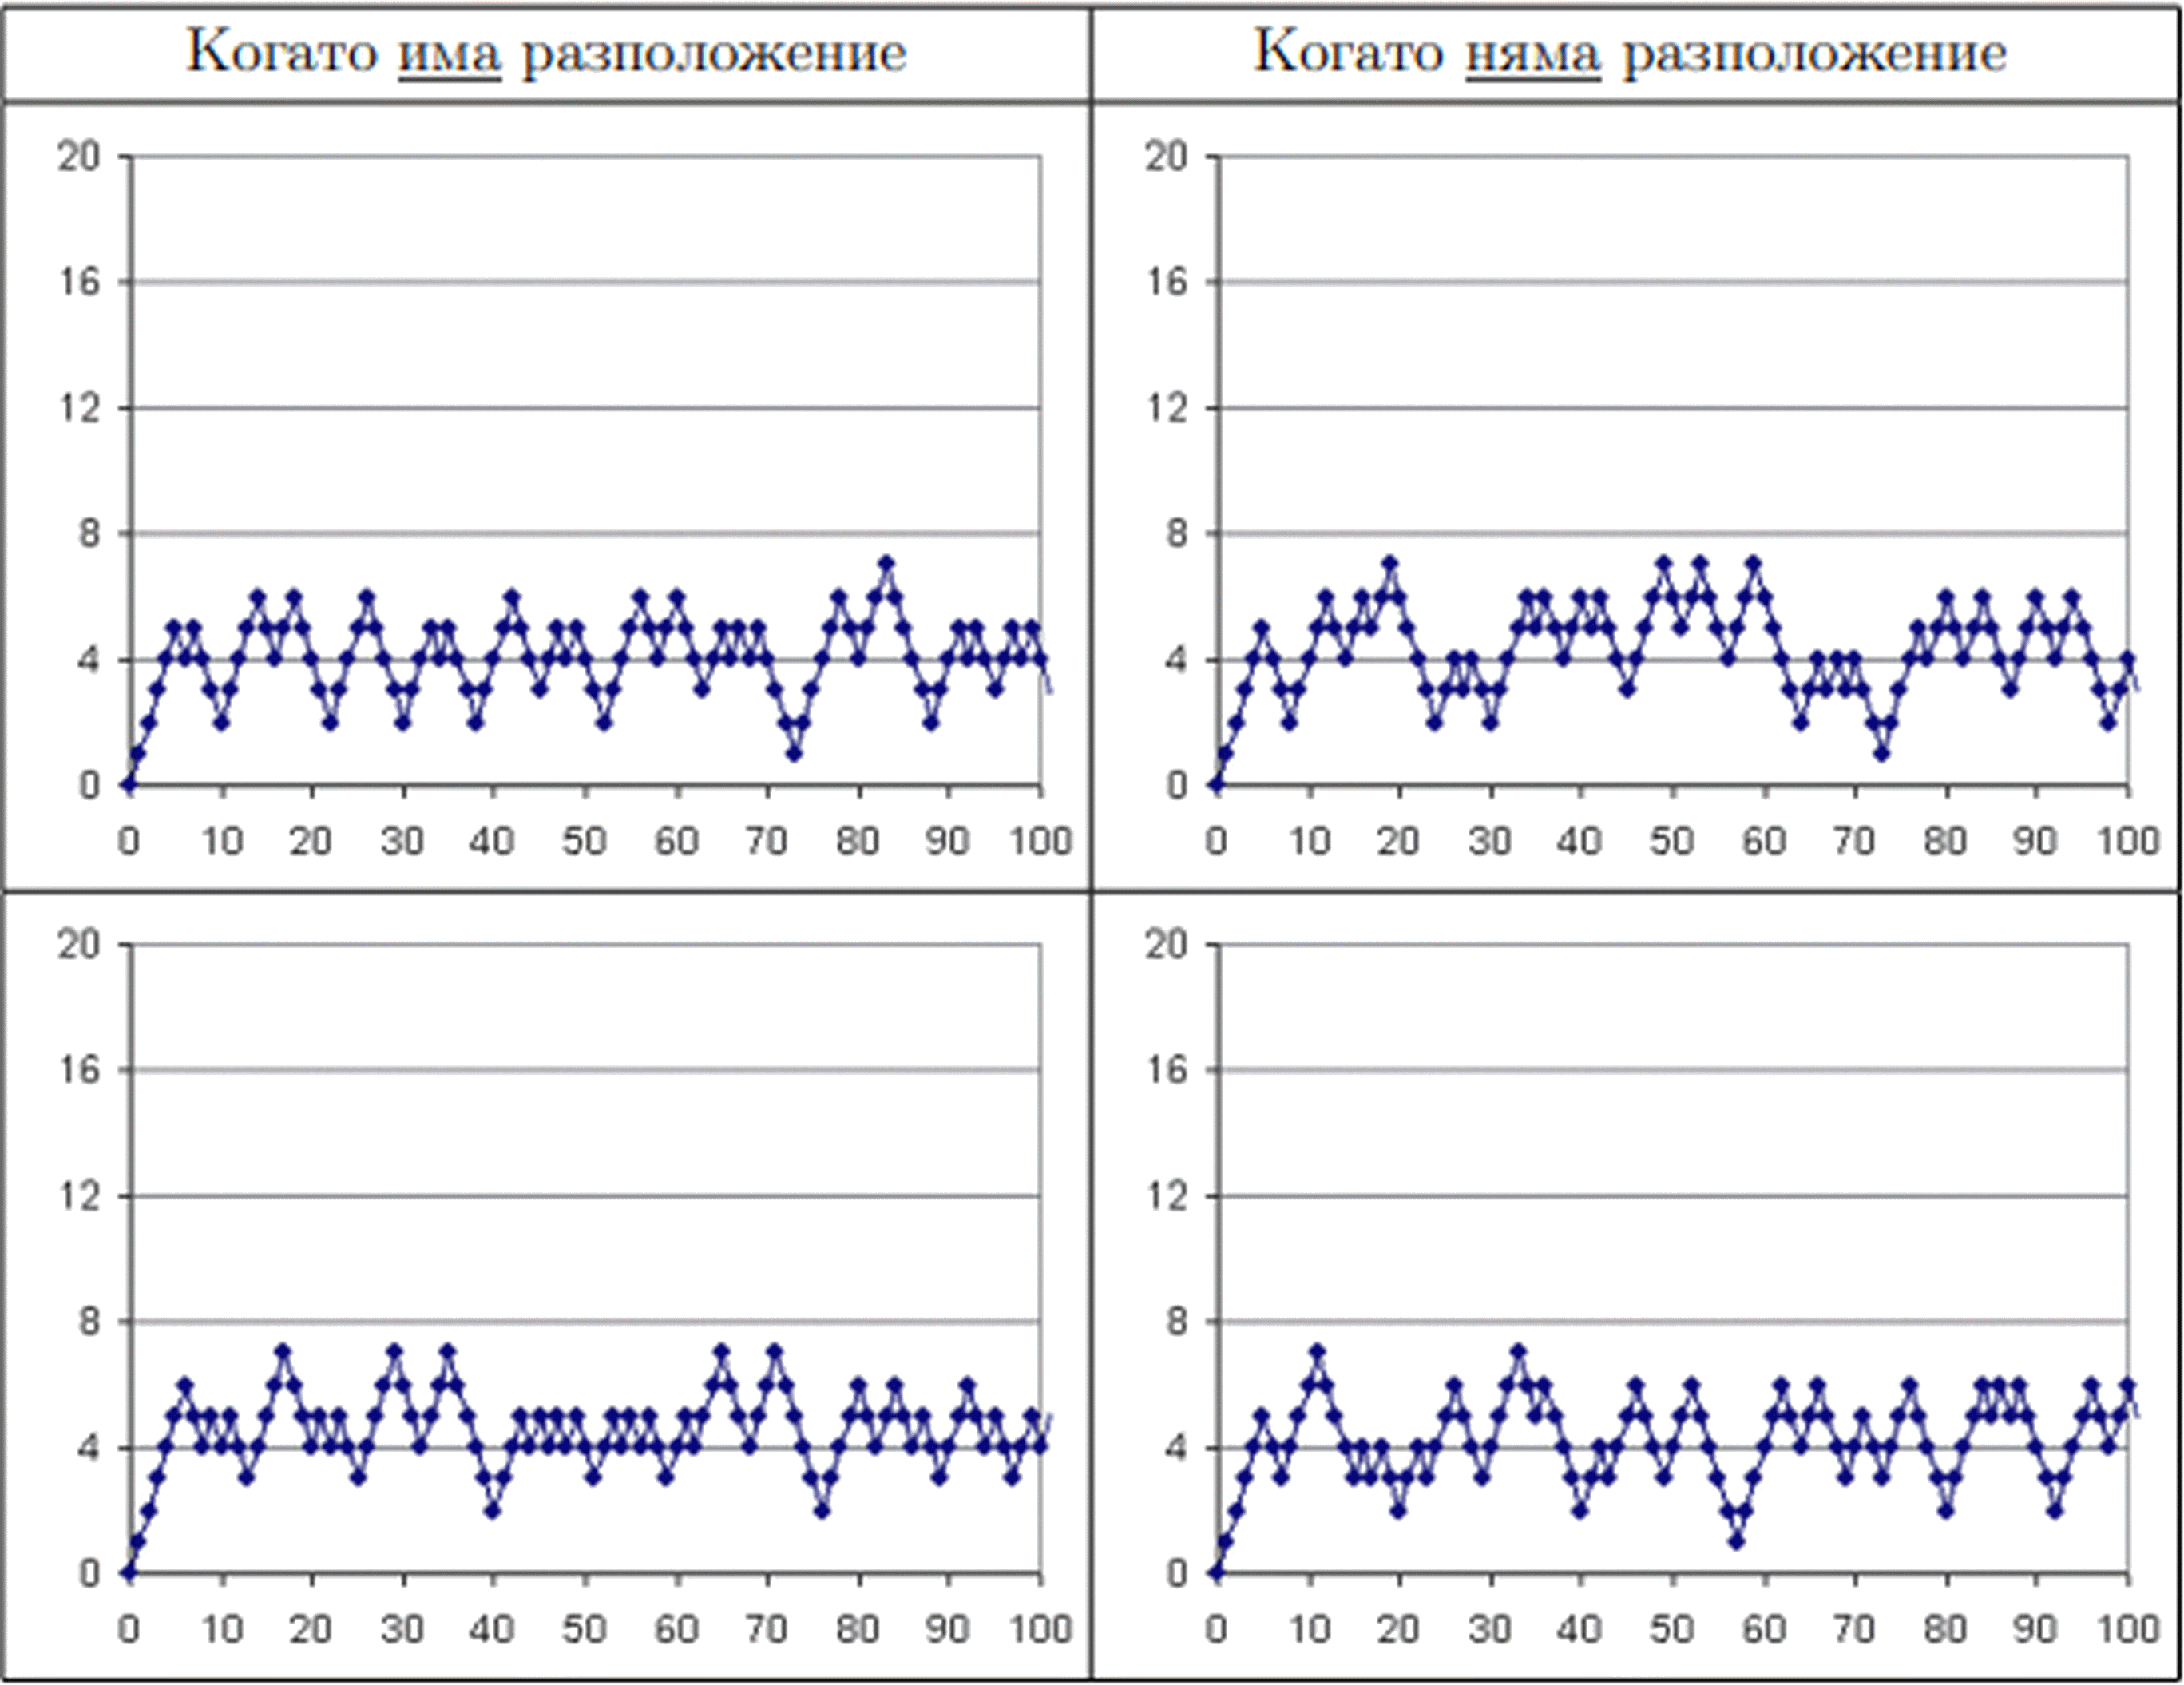
\includegraphics[scale=0.095]{queen_typ_mem8.png}
\end{frame}
\begin{frame}{Задача за цариците (експерименти)}
	Траектории на \mbox{$\left(\xi_{\,t}\right)_{t\geq 0}$}
	при дъска \mbox{$16 \times 16$} с критична плътност.\vspace{3pt}\\
	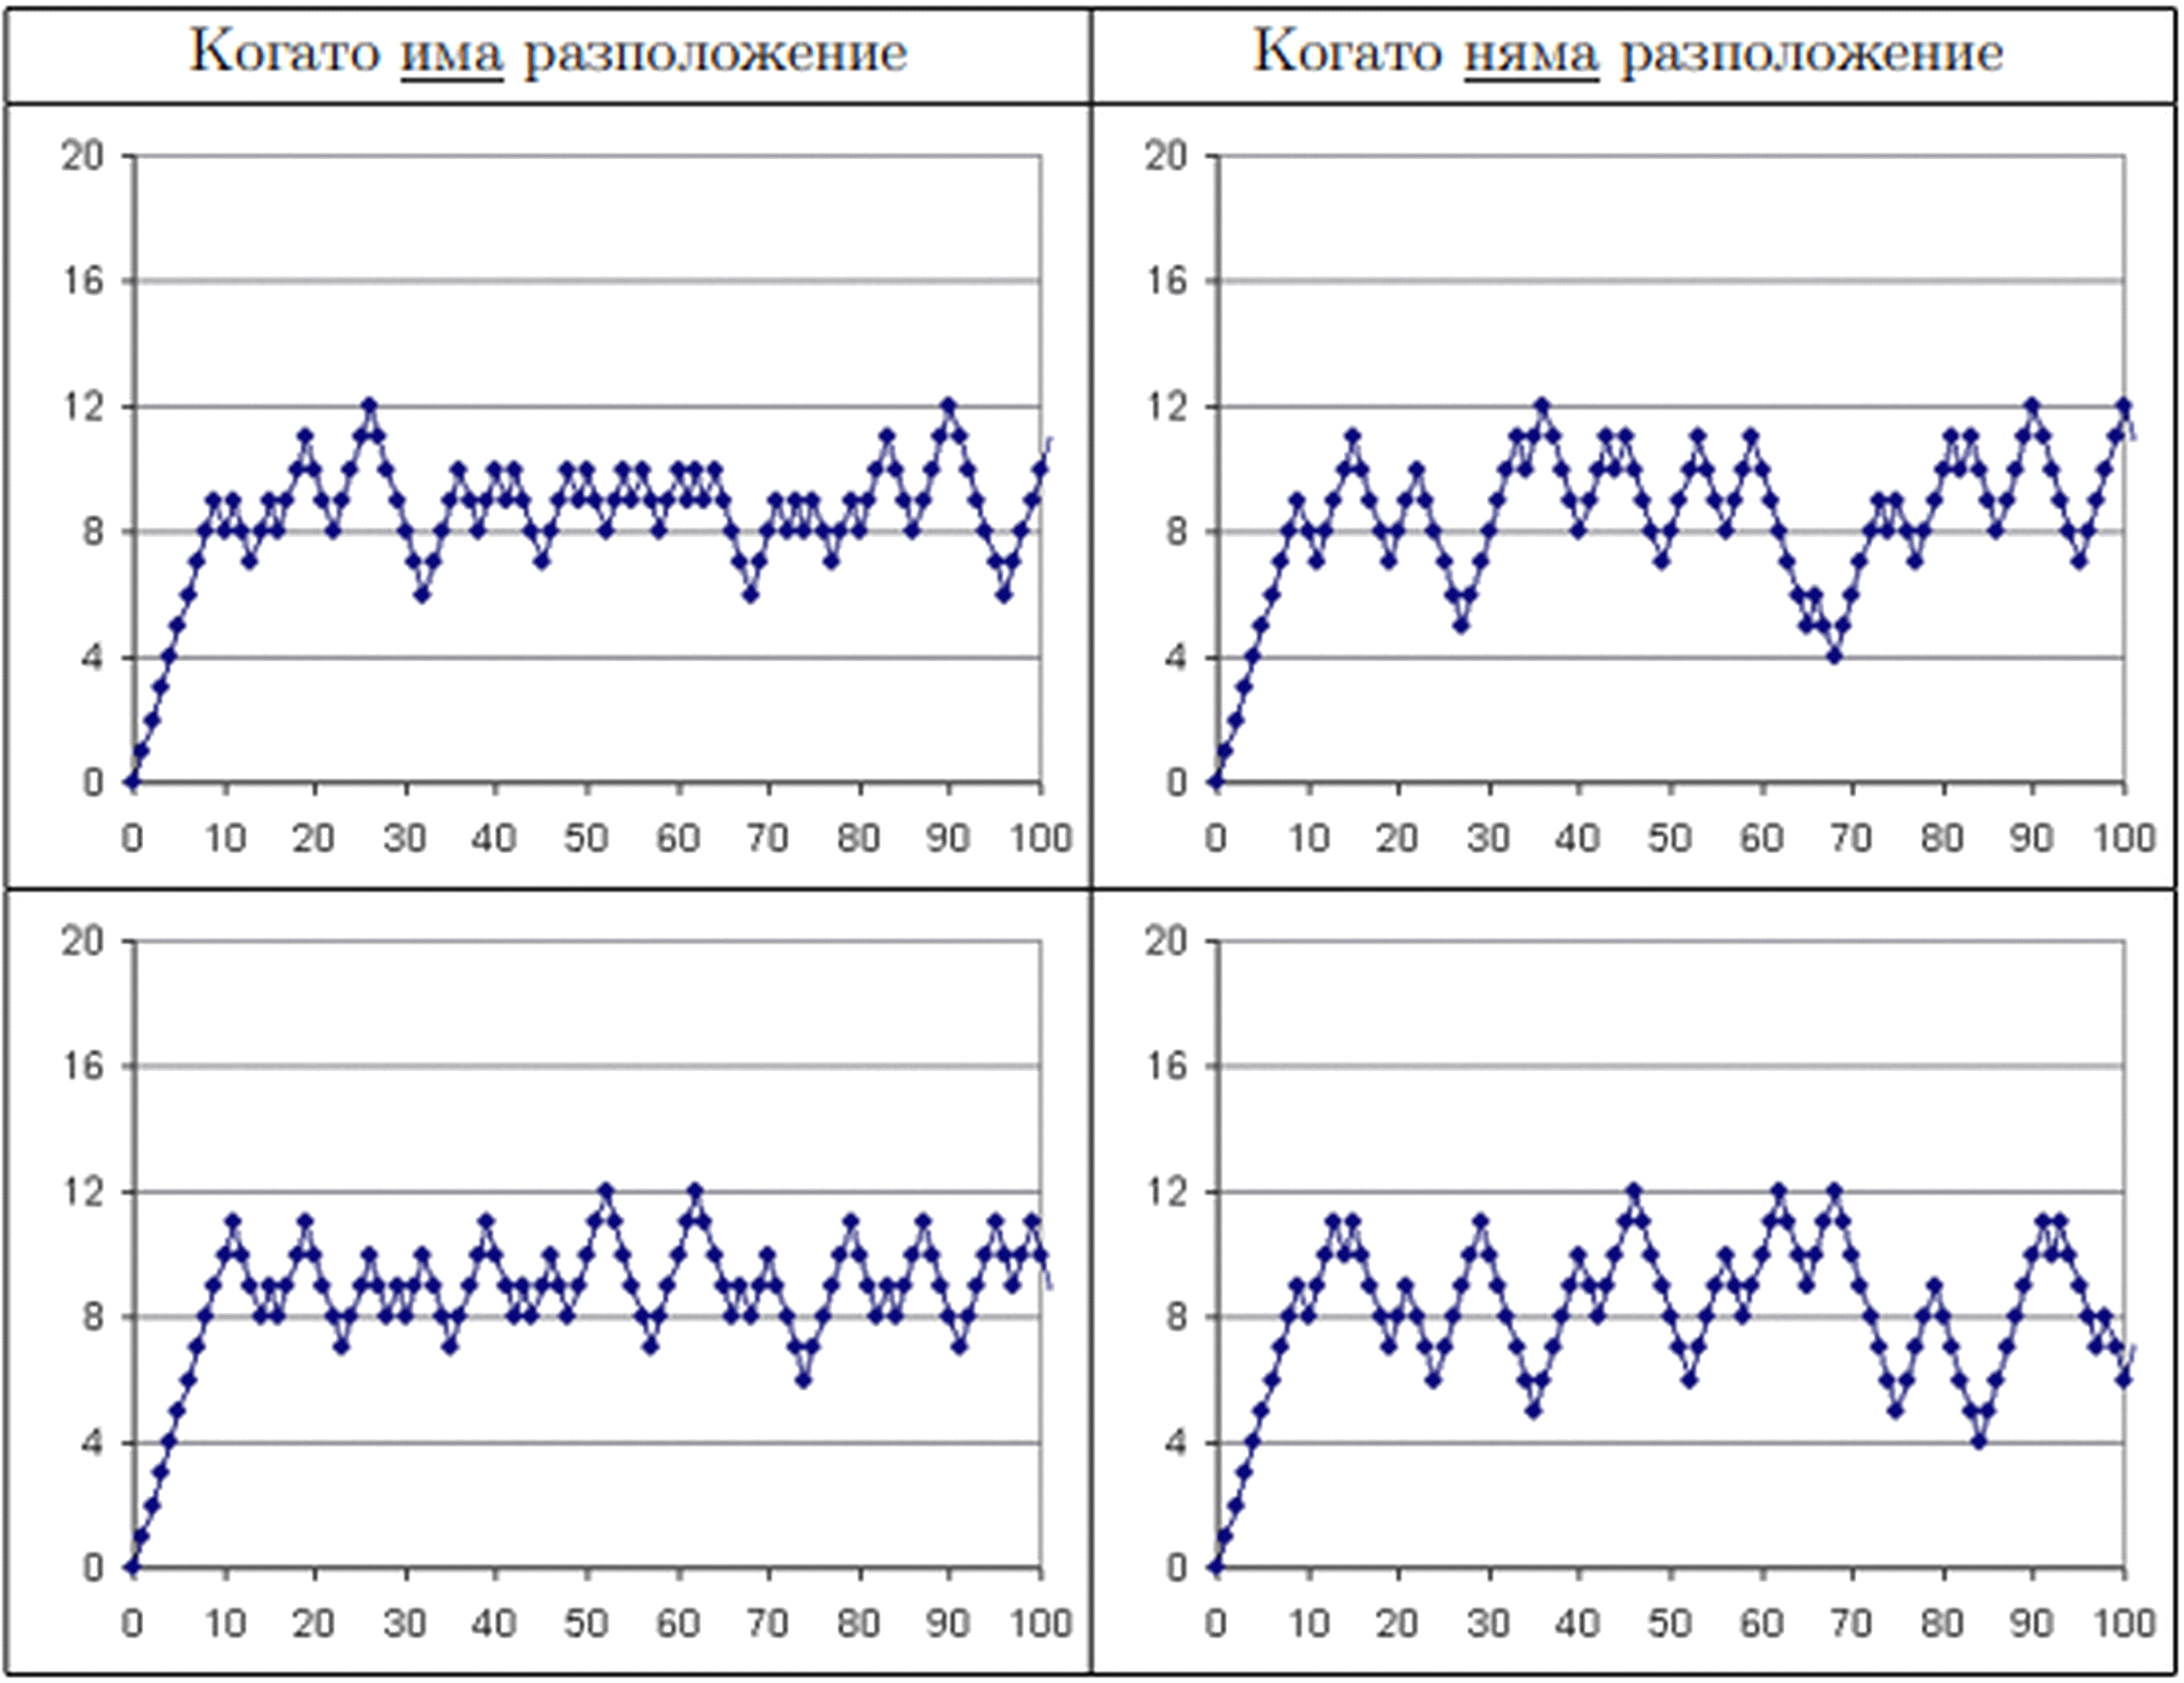
\includegraphics[scale=0.095]{queen_typ_mem16.png}
\end{frame}
\end{document}
